\section{角动量}

\subsection{角动量和力矩}

\begin{definition}[角动量]
    对于一个固定的参考点，定义一个质点的\textbf{角动量}为
    $$
    \vect{L} = \vect{r} \times \vect{p}
    $$
    其中 $\vect{r}$ 是质点关于参考点的位移，$\vect{p}$ 是质点的动量。
\end{definition}

角动量的变化量也称为\textbf{角冲量}或\textbf{冲量矩}。

\begin{definition}[力矩]
    对于一个固定的参考点，定义一个质点的\textbf{力矩}为
    $$
    \vect{M} = \vect{r} \times \vect{F}
    $$
    其中 $\vect{r}$ 是质点关于参考点的位移，$\vect{F}$ 是作用在质点上的力。
\end{definition}

\begin{theorem}[角动量定理]
    对于一个质点，其角动量的变化率等于作用在质点上的合外力矩，即
    $$
    \dv{\vect{L}}{t} = \vect{M}
    $$
\end{theorem}

对于质点组中两个质点 $i, j$，假设其中有一对作用力 $\vect{F}_{ij}$，那么其贡献的力矩：
$$
\vect{M}_{ij} = \vect{r}_i \times \vect{F}_{ij} + \vect{r}_j \times \vect{F}_{ji} = (\vect{r}_i - \vect{r}_j) \times \vect{F}_{ij}
$$
而 $\vect{F}_{ij}$ 沿 $\vect{r}_i - \vect{r}_j$ 方向，因此 $\vect{M}_{ij} = 0$。进一步得到，质点组的合内力矩为 $\vect{0}$。因此我们得到质点组的角动量变化定理：

\begin{theorem}[质点组的角动量变化定理]
    对于一个质点组，其角动量的变化率等于作用在质点组上的合外力矩，即
    $$
    \dv{\vect{L}}{t} = \vect{M}_{\text{外}}
    $$
\end{theorem}

\section{有心运动}

\begin{definition}[有心力与有心力场]
    \textbf{有心力}是指方向始终指向一个固定点的力，其大小仅依赖于质点到该点的距离。由有心力产生的力场称为\textbf{有心力场}。

    可以证明，有心力是保守力。
\end{definition}

对于一个有心力场中质量为 $m$ 的质点，其运动方程为：
$$
m \ddot{\vect{r}} = -F(\abs{\vect{r}}) \cdot \frac{\vect{r}}{\abs{\vect{r}}}
$$

\begin{theorem}[开普勒第二定律]
    在有心力场中，质点在任意相等时间间隔内扫过的面积相等。

    \begin{proof}
        对于有心力场中的质点，其角动量守恒，即
        $$
        \vect{L} = \vect{r} \times \vect{p} = m \vect{r} \times \vect{v} = \text{const}
        $$
        考察一个时间微元中掠过的面积：
        $$
        \begin{aligned}
            \dd{S} & = \abs{\frac{1}{2} (\vect{r} \times (\vect{r} + \dd{\vect{r}}))} \\
            & = \abs{\frac{1}{2} (\vect{r} \times \dd{\vect{r}})} \\
            & = \abs{\frac{1}{2} (\vect{r} \times \vect{v} \dd{t})} \\
            & = \abs{\frac{1}{2m} \vect{L}} \dd{t}
        \end{aligned}
        $$
        因此，$\dv{S}{t}$ 是常量。
    \end{proof}
\end{theorem}

\subsection{作业}

\begin{problem}
    习题 4.14
    \begin{solution}
        \begin{enumerate}
            \item[\textbf{1)}] 由题可知：
            $$
            \frac{m v_0^2}{R_0} = \frac{G M m}{R_0^2} \implies GM = v_0^2 R_0
            $$
            那么该行星的逃逸速度 $v_1$ 满足：
            $$
            \frac{1}{2} m v_1^2 = \frac{G M m}{R_0} \implies v_1 = \sqrt{\frac{2 G M}{R_0}} = \sqrt{2} v_0
            $$
            \item[\textbf{2)}] 设上抛速度为 $v_2$，那么：
            $$
            \frac{1}{2} m v_2^2 = \ab(-\frac{G M m}{2 R_0}) - \ab(-\frac{G M m}{R_0})
            $$
            解得 $v_2 = v_0$。
        \end{enumerate}
    \end{solution}
\end{problem}

\begin{problem}
    习题 4.16
    \begin{solution}
        \begin{enumerate}
            \item[\textbf{1)}]
            $$
            \begin{dcases}
                m v_A \sin 30^\circ - m v_B \sin 45^\circ = 0 \\
                m v_A \cos 30^\circ + m v_B \cos 45^\circ = m v_{A0}
            \end{dcases}
            $$
            解得 $v_A = 80\ab(\sqrt{3} - 1)\,\mathrm{m / s},\ v_B = 80\ab(\sqrt{6} - \sqrt{2})\,\mathrm{m / s}$。

            \item[\textbf{2)}]
            $$
            \eta = 1 - \frac{\frac{1}{2} m_A v_A^2 + \frac{1}{2} m_B v_B^2}{\frac{1}{2} m_A v_{A0}^2} = 3 \sqrt{3} - 5 \approx 19.6\%
            $$
        \end{enumerate}
    \end{solution}
\end{problem}

\begin{problem}
    习题 5.1
    \begin{solution}
        角动量：
        $$
        \begin{aligned}
            \vect{L} & = m \vect{r} \times \vect{v} \\
            & = m \ab(x \vect{e}_i + y \vect{e}_j) \times \ab(v_x \vect{e}_i + v_y \vect{e}_j) \\
            & = m (x v_y - y v_x) \vect{e}_i \times \vect{e}_j
        \end{aligned}
        $$
        力矩：
        $$
        \begin{aligned}
            \vect{M} & = \vect{r} \times \vect{F} \\
            & = \ab(x \vect{e}_i + y \vect{e}_j) \times \ab(-f \vect{e}_i) \\
            & = f y \vect{e}_i \times \vect{e}_j
        \end{aligned}
        $$
    \end{solution}
\end{problem}

\begin{problem}
    习题 5.4
    \begin{solution}
        \begin{figure}[H]
            \centering
            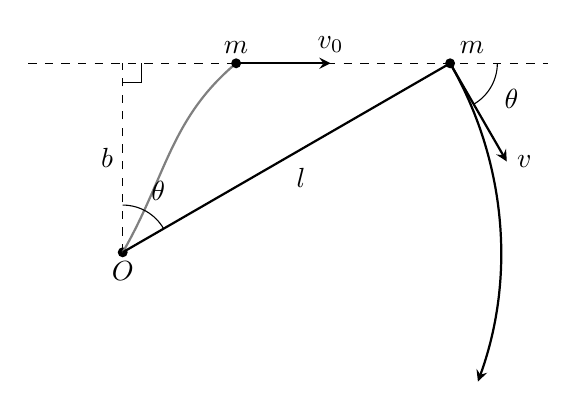
\begin{tikzpicture}[>=stealth, scale=1.2]
                \coordinate (O) at (0,0);
                \coordinate (H) at (0,2);
                \coordinate (M1) at (1.2,2);
                \coordinate (M2) at ({4*cos(30)}, 2);
                
                \fill (O) circle (1.5pt) node[below] {$O$};
                
                \draw[dashed] (-1,2) -- (4.5,2);
                \draw[dashed] (O) -- (H) node[midway, left] {$b$};
                \draw (0.2,2) -- (0.2,1.8) -- (0,1.8);
                
                \draw[thick, gray] (O) to[out=60, in=220] (M1);
                \fill (M1) circle (1.5pt) node[above] {$m$};
                \draw[->, thick] (M1) -- ++(1,0) node[above] {$v_0$};
                
                \draw[thick] (O) -- (M2) node[midway, below right] {$l$};
                \fill (M2) circle (1.5pt) node[above right] {$m$};
                
                \draw[thick, ->] (M2) arc (30:-20:4);
                \draw[->, thick] (M2) -- ++({1.2*cos(-60)}, {1.2*sin(-60)}) node[right] {$v$};
                
                \draw (0,0.5) arc (90:30:0.5);
                \node at (60:0.75) {$\theta$};
                
                \draw (M2) ++(0.5,0) arc (0:-60:0.5);
                \path (M2) ++(-30:0.75) node {$\theta$};
            \end{tikzpicture}
            \caption{$m$ 的运动示意}
        \end{figure}

        \begin{enumerate}
            \item[\textbf{1)}] 根据图示可知：
            $$
            v = v_0 \sin \ab(\frac{\pi}{2} - \theta) = v_0 \cos \theta = v_0 \frac{b}{l}
            $$
            因此：
            $$
            \frac{E_k'}{E_k} = \frac{\frac{1}{2} m v^2}{\frac{1}{2} m v_0^2} = \frac{b^2}{l^2}
            $$
            损失的能量转化为了绳子的内能。

            \item[\textbf{2)}] 绳断后质点不受力，做匀速直线运动，角动量保持不变。
        \end{enumerate}
    \end{solution}
\end{problem}